% !TEX encoding = UTF-8 Unicode
\documentclass[11pt, a4paper]{article}
\usepackage{authblk}
\linespread{1.2}
\usepackage{palatino}
\usepackage{parskip}
\usepackage{graphicx}
\usepackage{hyperref}


% Title
\title{Manual for tsRFinder}
\author{Qinhu Wang}
\author{Weixing Shan\thanks{Email: wxshan@nwafu.edu.cn}}
\affil{Northwest A\&F University}
\date{\today}


%%% Begin document
\begin{document}

\maketitle
\tableofcontents

\section{Introduction}

Small RNAs are key regulators of gene expression, such as miRNA, siRNA, and piRNA. The tRNA-derived small RNA (tsRNA), is a class of novel small RNA have been identified recently. However, there is no public tool available for tsRNA prediction yet. We thus developed tsRFinder for tsRNA prediction. It takes the raw data of small RNA sequencing reads and the reference genome sequence, and identify tsRNA for you automatically.

\section{How to install}

\subsection{Dependencies}

tsRFinder depends on the following programmes, please check and install them \footnote{The dependency versions were based on the oldest test enviroment we have.} at first:


\begin{itemize}

\item Perl, greater than v5.16.2, required, for tsRFinder.pl execution. And it was always installed already in most of the UNIX-like operating systems.
\item tRNAscan-SE, greater than v1.3.1, required, for tRNA prediction. \\http://lowelab.ucsc.edu/tRNAscan-SE
\item bowtie, greater than v1.0.0, required, for small RNA mapping. \\https://github.com/BenLangmead/bowtie
\item R, greater than v2.15.2, required, for small RNA data analysis and illustration. \\http://www.r-project.org
\item fastx\_toolkit, greater than v0.0.14, optional if you have already processed the raw sequencing data yourself. \\https://github.com/agordon/fastx\_toolkit

\end{itemize}

\subsection{Installation}

tsRFinder is maintained on GitHub and is ready-to-use, no compilation is required. However, if you take some time to improve the configuration, it may save you a lot of time for trouble shooting.

First, you can clone \footnote{If git is not installed, download it from http://git-scm.com} tsRFinder by typing:

{\small \begin{verbatim}
git clone https://github.com/wangqinhu/tsRFinder.git
\end{verbatim}}

in the terminal, alternatively, you can download it from

{\small \begin{verbatim}
https://codeload.github.com/wangqinhu/tsRFinder/zip/master
\end{verbatim}
}

and then unzip master file.

When tsRFinder is cloned or unpacked, move the entire directory to an proper place and add the tsRFinder path to the environment. For example, if tsRFinder is placed in /your/path/of/tsRFinder, then type the following in the terminal if you are using bash.

{\small \begin{verbatim}
echo export PATH="/your/path/of/tsRFinder:$PATH" >> ~/.bashrc
echo export tsR_dir="/your/path/of/tsRFinder" >> ~/.bashrc
source ~/.bashrc
\end{verbatim}}

And now, you can running tsRFinder for your dataset.

\section{How to use}

\subsection{Preparation the dataset}

Before running tsRFinder, you are asked to prepare/download the following two files: (1) the reference genome sequence, or the reference tRNA sequence and, (2) the small RNA reads.

We strongly recommend you using the reference genome sequence and the raw small RNA sequencing data, since tsRFinder can help you prepare the reference tRNA data and clean small RNA data automatically. If you want to prepare the tRNA file and small RNA reads file by yourself, you can running the demo data and then find what exact format of tRNA reference and small RNA reads file can be accepted instead, this is allowed by not encouraged. 

\subsection{Running the pipeline}

tsRFinder supplies two ways for inputs, you can use both configuration file or command line option. We recommend you use a command line option for debugging and building your configuration file. Once your inputs had been determined, you can write it to a configuration file for your analysis.

If tsRFinder is properly installed, you can run tsRFinder from your terminal directly, see the usage below.

{\small \begin{verbatim}
tsRFinder usage:

    tsRFinder.pl <option>

    -c  Configuration file
    -l  Label
    -g  Reference genomic sequence
    -t  Reference tRNA sequence
    -s  Small RNA sequence
    -a  Adaptor sequence
    -n  Min read length
    -x  Max read length
    -h  Help
    -v  Version

Example:

    tsRFinder.pl -c demo/tsR.conf
\end{verbatim}}

\section{Demo}

\subsection{Demo data}

\textbf{Demo refseq}: we used serval random sequences embedded with some real tRNA as a pseudo reference genome sequence. This small sequence data in fasta format can be accessed in the file "tsRFinder/demo/genome.fa". In your analysis, if you have a reference genome, just replace it with the reference sequence; if you don't have reference genome sequence, you can use the reference tRNA sequence instead. Figure \ref{refseq} shows what a refseq file look like.

\begin{figure}[htbp]
\begin{center}
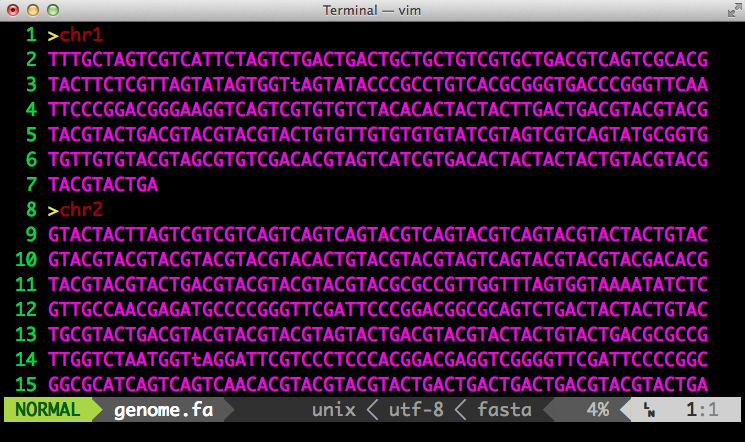
\includegraphics[width=12cm]{refseq.png}
\caption{Screenshot of the reference sequence in fasta format} 
\label{refseq}
\end{center}
\end{figure}

\textbf{Demo sRNA}: we extracted a bit of raw reads from some real experimental data as a demo here. Each read of the raw small RNA data have 4 lines, just like what we have show in Figure \ref{fastq}.

\begin{figure}[htbp]
\begin{center}
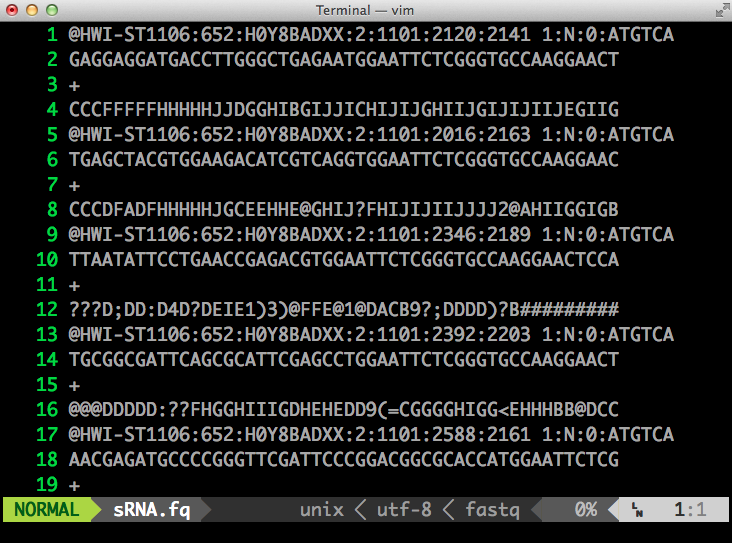
\includegraphics[width=12cm]{fastq.png}
\caption{Screenshot of the small RNA sequence in fastq format} 
\label{fastq}
\end{center}
\end{figure}

\subsection{Demo running}

tsRFinder allowes you specify your inputs via a separate configuration file, for example, here is the content our demo tsR.conf:

\begin{verbatim}
label               :  Abc
reference_genome    :  demo/genome.fa 
reference_tRNA      :  NA
sRNA                :  demo/sRNA.fq
adaptor             :  TGGAATTCTCGGGTGCCAAGG
min_read_length     :  18
max_read_length     :  45
\end{verbatim}

Currently we have 7 arguments used for filling. The argument items and the inputs are separated by colon (":"). We recommend you using the first three letters of the organism you are analysing as a label (e.g. for \textit{Arabidopsis thaliana} we use \textit{Ath}); the paths of reference genome and small RNA should be also supplied at least. If you are using a raw sequence data, please also input the adaptor sequence, and the shortest read you want to keep. If you are not using a reference tRNA prepared by yourself, leave this argument to "NA" please.

Once your configuration file is well prepared, typing the following in the terminal to run tsRFinder. In this demo, the configuration file is at demo/tsR.conf, so we write like this:

\begin{verbatim}
# We have set "tsR_dir" as an environment variable before
cd tsR_dir
./tsRFinder.pl -c demo/tsR.conf
\end{verbatim}

\subsection{Demo output}

By default, tsRFinder will give you a summary of which files have been outputted and some basic statistic. The predicted or user inputed tRNA sequence, the small RNA clean data, the tRNA reads, and the predicted tsRNA sequence were listed. Meanwhile, tsRFinder gives you additional summary on tRNA/tsRNA expression (including 5' tsRNA and 3' tsRNA), the text map (tmap) of small RNA mapped to tRNA, also graphics showing the expression evaluated by small RNA data. Additional, tsRFinder supplies a figure showing the small RNA and tRNA reads length distribution (Figure \ref{distribution}) for you.

See our demo summary here:

{\small \begin{verbatim}
---------
 SUMMARY 
---------

    tRNA seq : /Users/wangqinhu/tsRFinder/Abc/tRNA.fa
       Total : 5

  sRNA reads : /Users/wangqinhu/tsRFinder/Abc/sRNA.fa
       Total : 12432
      Unique : 7412

  tRNA reads : /Users/wangqinhu/tsRFinder/Abc/tRNA.read.fa
       Total : 286
      Unique : 52

   tsRNA seq : /Users/wangqinhu/tsRFinder/Abc/tsRNA.seq
       Total : 7
      Unique : 6

tsRNA report : /Users/wangqinhu/tsRFinder/Abc/tsRNA.report.xls

    text map : /Users/wangqinhu/tsRFinder/Abc/tsRNA.tmap

  visual map : /Users/wangqinhu/tsRFinder/Abc/images

distribution : /Users/wangqinhu/tsRFinder/Abc/distribution.pdf

stat. by BDI :
 Sensitivity : 0.940025252525252
 Specificity : 0.783809523809524
    Accuracy : 0.876447574334898

---------
\end{verbatim}
}

\begin{figure}[htbp]
\begin{center}
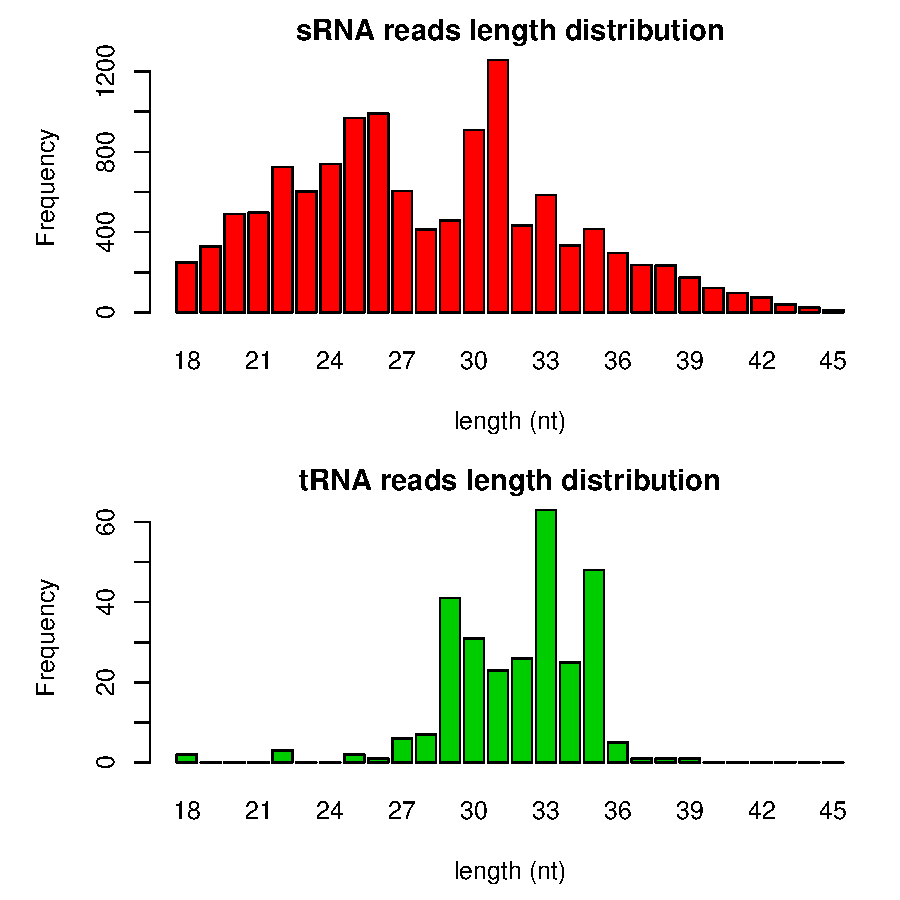
\includegraphics[width=12cm]{distribution.pdf}
\caption{Small RNA and tRNA reads distribution}
\label{distribution}
\end{center}
\end{figure}

\subsection{Visualization of tmap data}

To examine the map the tsRNA, we developed a vim syntax plugin for visualization (Figure \ref{tmap}). If you want to enable color text map, copy lib/tmap.vim into your vim syntax folder, and put the following line into your .vimrc file:

\begin{verbatim}
au BufNewFile,BufRead *.tmap  setf tmap
\end{verbatim}

When tmap.vim is correctly installed, open the tsRNA.tmap file with vim you will obtain a color text map, like this:

\begin{verbatim}
vim tsRNA.tmap
\end{verbatim}

\begin{figure}[htbp]
\begin{center}
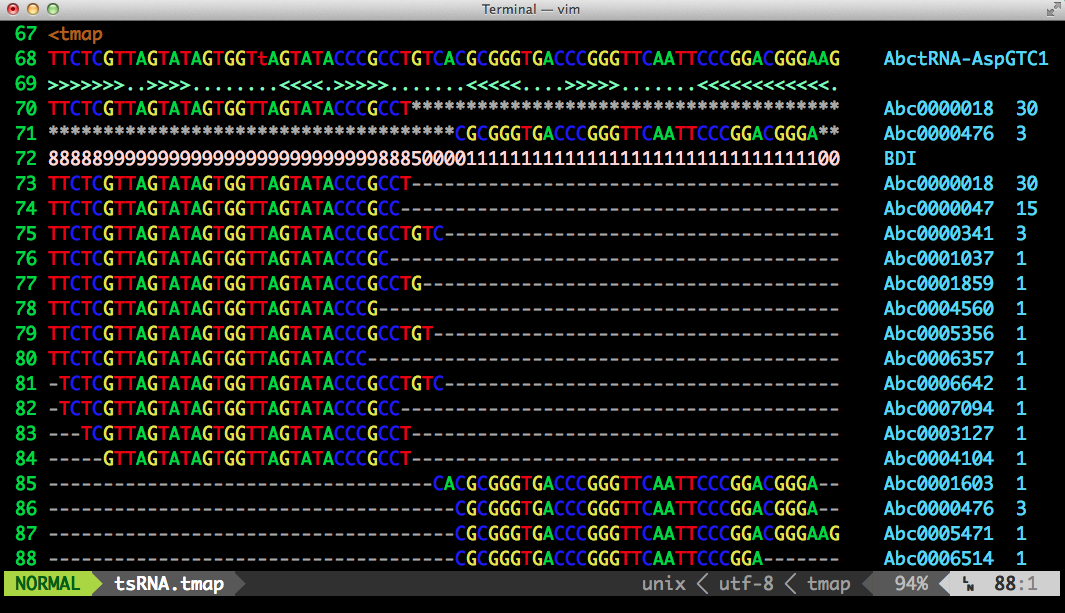
\includegraphics[width=12cm]{tmap.png}
\caption{Screenshot of color tmap} 
\label{tmap}
\end{center}
\end{figure}

If you prefer plain text view without highlighting, just open tsRNA.tmap with any kind of text editors you have.

\section{FAQ}

\textbf{1. Can tsRFinder running on Windows?}

No. tsRFinder used some build-in program of UNIX-like systems, for example, awk, grep and head, thus running on Windows may lead unexpected errors, we strongly recommend you running tsRFinder on Linux or OS X.

\textbf{2. What's the length required for small RNA reads?}

We recommend you sequencing from 15 - 50 nt for small RNA, however, 18 - 30 nt is OK if your tsRNA is less than 30 nt (such as tRF).

\textbf{3. I have problem in installing tsRFinder and/or the dependencies, where to get more help?}

You can create new issue for tsRFinder repository on GitHub. The URL is https://github.com/wangqinhu/tsRFinder/issues/new

\textbf{4. Where to report bugs?}

Goto https://github.com/wangqinhu/tsRFinder/issues/new

\textbf{5. Can we use tsRFinder for commercial purpose?}

Yes. tsRFinder is free, open source software, see the MIT license.

\end{document}
